% Created by tikzDevice version 0.10.1 on 2018-02-09 14:48:38
% !TEX encoding = UTF-8 Unicode
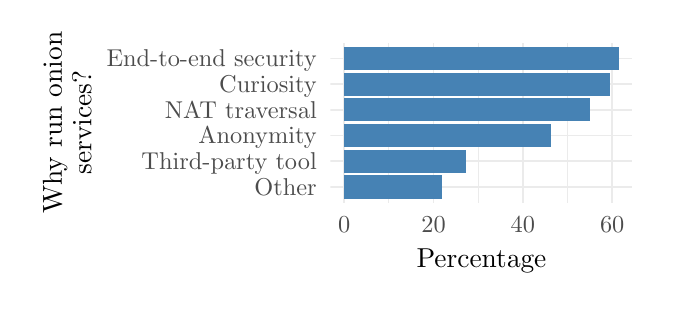
\begin{tikzpicture}[x=1pt,y=1pt]
\definecolor{fillColor}{RGB}{255,255,255}
\path[use as bounding box,fill=fillColor,fill opacity=0.00] (0,0) rectangle (224.04, 93.95);
\begin{scope}
\path[clip] (109.42, 30.77) rectangle (218.54, 88.45);
\definecolor{drawColor}{gray}{0.92}

\path[draw=drawColor,line width= 0.3pt,line join=round] (130.52, 30.77) --
	(130.52, 88.45);

\path[draw=drawColor,line width= 0.3pt,line join=round] (162.80, 30.77) --
	(162.80, 88.45);

\path[draw=drawColor,line width= 0.3pt,line join=round] (195.08, 30.77) --
	(195.08, 88.45);

\path[draw=drawColor,line width= 0.6pt,line join=round] (109.42, 36.35) --
	(218.54, 36.35);

\path[draw=drawColor,line width= 0.6pt,line join=round] (109.42, 45.66) --
	(218.54, 45.66);

\path[draw=drawColor,line width= 0.6pt,line join=round] (109.42, 54.96) --
	(218.54, 54.96);

\path[draw=drawColor,line width= 0.6pt,line join=round] (109.42, 64.26) --
	(218.54, 64.26);

\path[draw=drawColor,line width= 0.6pt,line join=round] (109.42, 73.57) --
	(218.54, 73.57);

\path[draw=drawColor,line width= 0.6pt,line join=round] (109.42, 82.87) --
	(218.54, 82.87);

\path[draw=drawColor,line width= 0.6pt,line join=round] (114.38, 30.77) --
	(114.38, 88.45);

\path[draw=drawColor,line width= 0.6pt,line join=round] (146.66, 30.77) --
	(146.66, 88.45);

\path[draw=drawColor,line width= 0.6pt,line join=round] (178.94, 30.77) --
	(178.94, 88.45);

\path[draw=drawColor,line width= 0.6pt,line join=round] (211.22, 30.77) --
	(211.22, 88.45);
\definecolor{fillColor}{RGB}{70,130,180}

\path[fill=fillColor] (114.38, 32.17) rectangle (149.80, 40.54);

\path[fill=fillColor] (114.38, 41.47) rectangle (158.47, 49.84);

\path[fill=fillColor] (114.38, 50.77) rectangle (189.17, 59.15);

\path[fill=fillColor] (114.38, 60.08) rectangle (203.34, 68.45);

\path[fill=fillColor] (114.38, 69.38) rectangle (210.43, 77.75);

\path[fill=fillColor] (114.38, 78.68) rectangle (213.58, 87.06);
\end{scope}
\begin{scope}
\path[clip] (  0.00,  0.00) rectangle (224.04, 93.95);
\definecolor{drawColor}{gray}{0.30}

\node[text=drawColor,anchor=base east,inner sep=0pt, outer sep=0pt, scale=  0.88] at (104.47, 33.32) {Other};

\node[text=drawColor,anchor=base east,inner sep=0pt, outer sep=0pt, scale=  0.88] at (104.47, 42.63) {Third-party tool};

\node[text=drawColor,anchor=base east,inner sep=0pt, outer sep=0pt, scale=  0.88] at (104.47, 51.93) {Anonymity};

\node[text=drawColor,anchor=base east,inner sep=0pt, outer sep=0pt, scale=  0.88] at (104.47, 61.23) {NAT traversal};

\node[text=drawColor,anchor=base east,inner sep=0pt, outer sep=0pt, scale=  0.88] at (104.47, 70.54) {Curiosity};

\node[text=drawColor,anchor=base east,inner sep=0pt, outer sep=0pt, scale=  0.88] at (104.47, 79.84) {End-to-end security};
\end{scope}
\begin{scope}
\path[clip] (  0.00,  0.00) rectangle (224.04, 93.95);
\definecolor{drawColor}{gray}{0.30}

\node[text=drawColor,anchor=base,inner sep=0pt, outer sep=0pt, scale=  0.88] at (114.38, 19.76) {0};

\node[text=drawColor,anchor=base,inner sep=0pt, outer sep=0pt, scale=  0.88] at (146.66, 19.76) {20};

\node[text=drawColor,anchor=base,inner sep=0pt, outer sep=0pt, scale=  0.88] at (178.94, 19.76) {40};

\node[text=drawColor,anchor=base,inner sep=0pt, outer sep=0pt, scale=  0.88] at (211.22, 19.76) {60};
\end{scope}
\begin{scope}
\path[clip] (  0.00,  0.00) rectangle (224.04, 93.95);
\definecolor{drawColor}{RGB}{0,0,0}

\node[text=drawColor,anchor=base,inner sep=0pt, outer sep=0pt, scale=  0.99] at (163.98,  7.44) {Percentage};
\end{scope}
\begin{scope}
\path[clip] (  0.00,  0.00) rectangle (224.04, 93.95);
\definecolor{drawColor}{RGB}{0,0,0}

\node[text=drawColor,rotate= 90.00,anchor=base,inner sep=0pt, outer sep=0pt, scale=  0.99] at ( 12.32, 59.61) {Why run onion};

\node[text=drawColor,rotate= 90.00,anchor=base,inner sep=0pt, outer sep=0pt, scale=  0.99] at ( 23.01, 59.61) {services?};
\end{scope}
\end{tikzpicture}
